\section{\ExercisePrefixEmbeddedC Display ansteuern \optional}
In diesem Abschnitt lernst du die Ansteuerung des Displays kennen.
Das Display hat eine Auflösung von 480 * 320 Pixeln.
Zunächst wirst du den Bildschirm in verschiedene Farben ausfüllen und die dafür benötigte Farbcodierung kennenlernen.
Anschließend wirst du Funktionen implementieren, um auf dem Bildschirm regelmäßige Muster und Texte auszugeben.
Alle in dieser Aufgabe verwendeten Funktionen müssen in der Datei \filename{display.c} implementiert werden. 
\Cref{tab:displayFunctions} dokumentiert zu das erwartete Verhalten der zu implementierenden Funktionen.
%
\begin{table}
	\centering
	\caption{Wichtige Funktionen und Variablen für das Display}
	\label{tab:displayFunctions}
	\begin{tabular}{p{7cm}p{7cm}}
        \toprule
		\textbf{Funktionen/Variablen} & \textbf{Beschreibung} \\
        \midrule
        \lstinline|void drawRect(int16_t x, int16_t y, int16_t w, int16_t h, uint16_t color)|
        & Zeichnet die Umrandung eines Rechtecks in der Farbe color mit der Breite w und der Höhe h an die Stelle x,y. \\ \hline
		\lstinline|void fillRect(int x1, int y1, int w, int h, uint16_t fillcolor)|
        & Zeichnet ein ausgefülltes Rechteck in der Farbe fillcolor mit der Breite w und der Höhe h an die Stelle x,y. \\ \hline
		\lstinline|void drawPixel(int16_t x, int16_t y, uint16_t color)|
        & Zeichnet ein Pixel an x,y mit der Farbe color. \\ \hline
		\lstinline|void fillScreen(uint16_t color)| 
        & Füllt den gesamten Bildschirm mit der Farbe color. \\ \hline
		\lstinline|uint16_t color565(uint8_t r, uint8_t g, uint8_t b)|
        & Umwandlung von RGB in HEX 565. \\
        \bottomrule
	\end{tabular}
\end{table}

\subsection{Bildschirm umfärben}
Das Display verwendet eine RGB565-Codierung für Farben (auch als \enquote{High Color} bekannt\footnote{\url{https://en.wikipedia.org/wiki/High_color}}).
Bei der RGB565-Codierung werden 5 Bits für Rot, 6 Bits für Grün und 5 Bits für Blau verwendet (siehe \Cref{fig:rgb565})
%
\begin{figure}
    \begin{centering}
        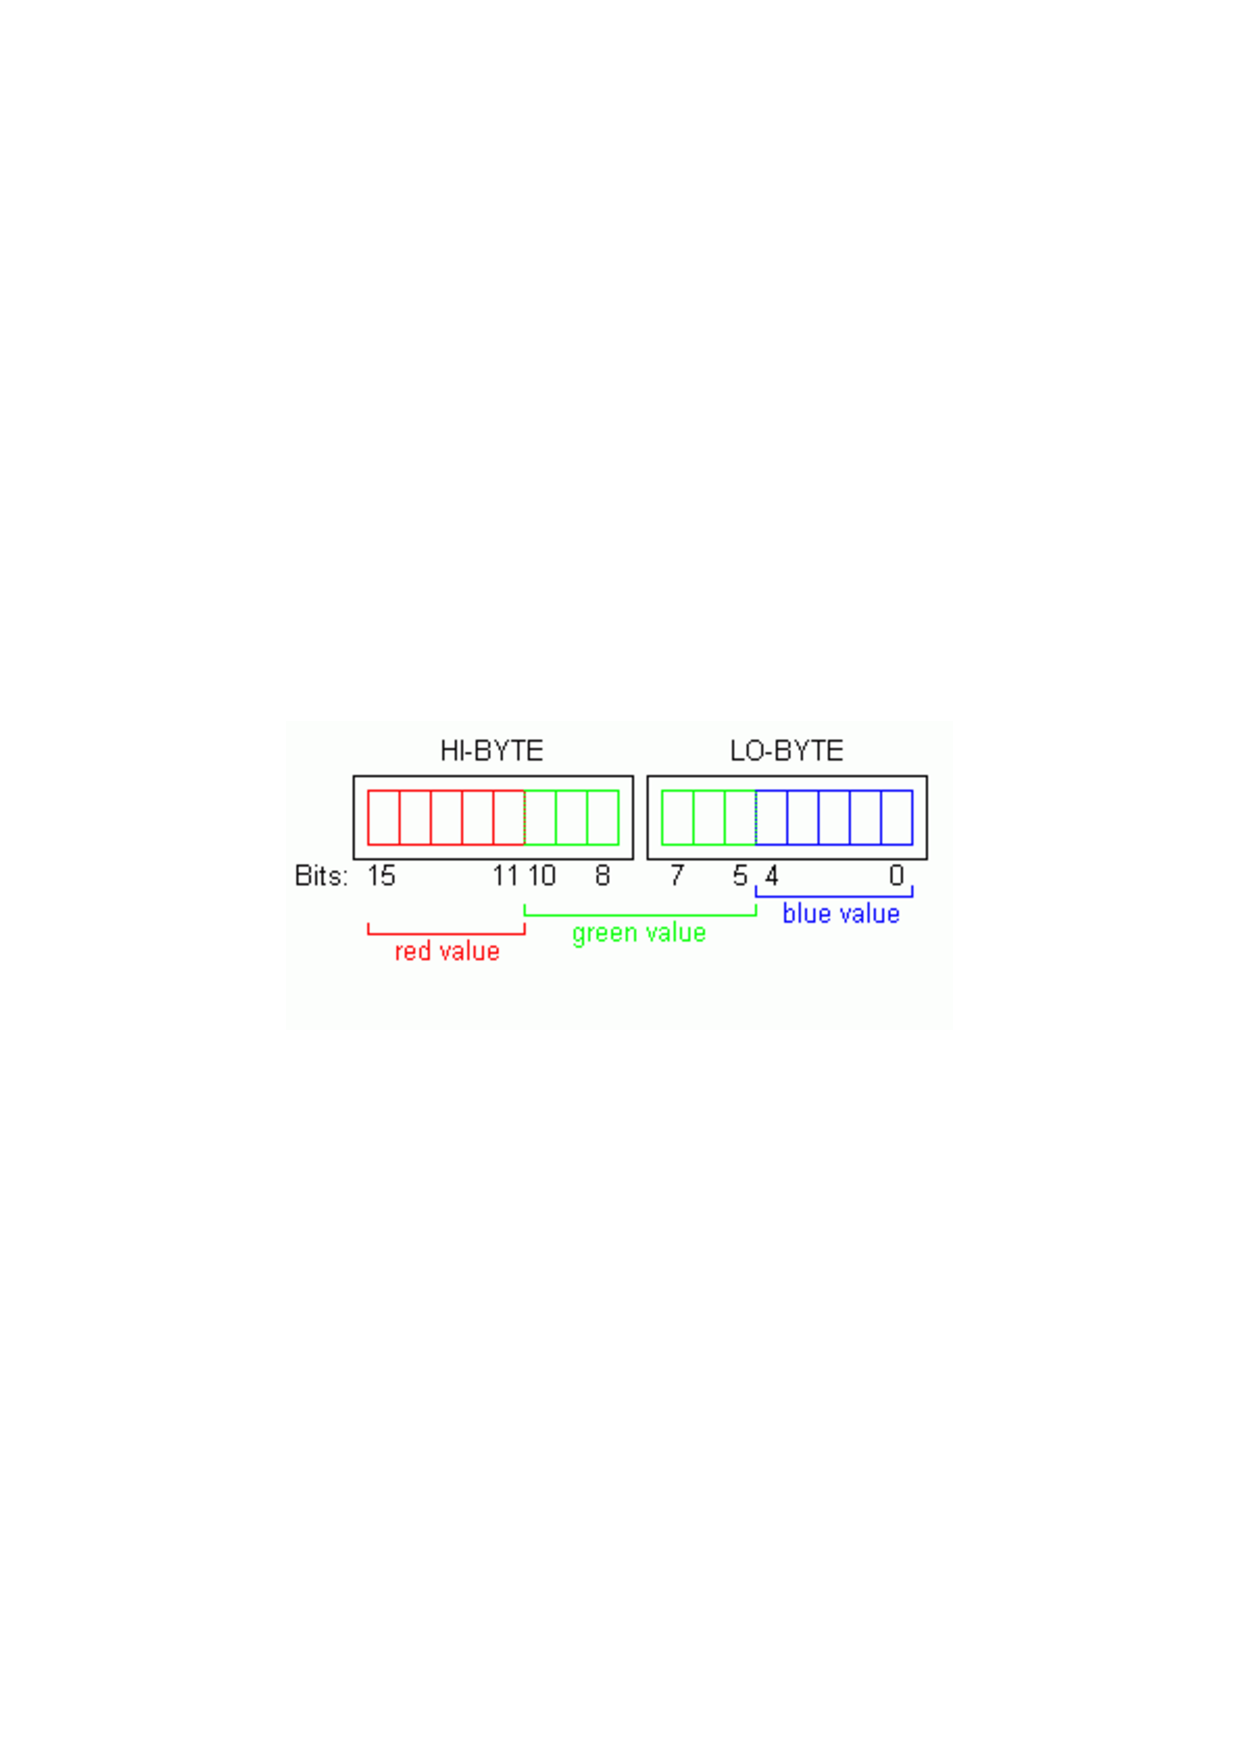
\includegraphics[width=.5\textwidth]{./05_c/figures/rgb565}
        \caption{RGB565 Codierung}
        \label{fig:rgb565}
    \end{centering}
\end{figure}
%
Um auch eigene Farben nutzen zu können, implemnetierst du zunächst die Funktion \lstinline|color565(uint8_t r, uint8_t g, uint8_t b)|, welche RGB888-Farben in RGB565-Farben umzuwandelt.
Der Umwandlungsalgorithmus arbeitet für drei gegebene Bytes (\lstinline|uint8_t| oder \lstinline|unsigend char|) \lstinline|r, g, b| wie folgt:
\begin{enumerate}
\item 
Extrahiere die höchstwertigen 5 Bits von \lstinline|r|, die höchstwertigen 6 Bits von \lstinline|g| und die höchstwertigen 5 Bits von \lstinline|b|.
Nutze den Bit-Und-Operator mit einer passenden Bitmaske, um nur die entsprechenden Bits beizubehalten und alle anderen Bits auf 0 zu setzen.
Verwende anschließend den Shift-Operator, um die extrahierten Bits ans untere Ende des Bytes zu schieben.
Es folgt eine Skizze für den Rot-Kanal.
\begin{lstlisting}
uint8_t r          = 0xA7;   // --> 0b10100111
uint8_t hiR        = r ______; // --> 0x00A0; 0b10100000
uint8_t hiRShifted = r ______; // --> 0x0014; 0b00010100
\end{lstlisting}
\item 
Füge die extrahierten Bits mittels des Bit-Oder-Operators zusammen, um den RGB565-Wert zu erhalten:
Beachte dabei, dass du mithilfe des Links-Shift-Operators die einzelnen Teile korrekt ausrichtest.
Beispielsweise muss \lstinline|hiRShifted| vor der Veroderung um 11 Bits nach links verschoben werden.
Beachte, dass das Ergebnis 16 Bit lang sein muss und wir deshalb den Typ \lstinline|uint16_t| verwenden.
\begin{lstlisting}
uint16_t result = (hiRShifted ____) | (hiGShifted ____ ) | (hiBShifted ____);
\end{lstlisting}
\end{enumerate}
Zum Testen deiner Implementation kannst du die Vergleichswerte in \Cref{tab:rgb565Table} nutzen.
\begin{table}[]
	\centering
	\caption{RGB565-Farbwerte}
	\label{tab:rgb565Table}
	\begin{tabular}{lll}
        \toprule
		\textbf{Farbe} & \textbf{RGB888} & \textbf{RGB565} \\
        \midrule
		Cyan   & \lstinline|0x00EAFF| & \lstinline|0x075F| \\
		Rosa   & \lstinline|0xFC00FF| & \lstinline|0xF81F| \\
		Orange & \lstinline|0xFFB400| & \lstinline|0xFDA0| \\
        \bottomrule
	\end{tabular}
\end{table}
Gehe dazu wie folgt vor:
\begin{enumerate}
\item 
Lege dir eine leere \lstinline|main|-Funktion an und binde den Header \filename{display.h} ein.
\item 
Füge die folgende Zeile ein, um deinen Code für die Farbe Cyan zu testen.
\end{enumerate}
\RKi{Beschreiben, wie man das mithilfe Debuggers macht.}
Die Datei \filename{display.h} enthält außerdem einige vordefinierten Farben, die du ebenfalls bei den folgenden Aufgaben nutzen kannst: \lstinline|BLACK| (\lstinline|0x0000|), \lstinline|BLUE| (\lstinline|0x001F|), \lstinline|RED| (\lstinline|0xF800|), \lstinline|GREEN| (\lstinline|0x07E0|), \lstinline|YELLOW| (\lstinline|0xFFE0|), \lstinline|WHITE| (\lstinline|0xFFFF|).


\subsection{Regelmäßiges Muster ausgeben}
In diesem Abschnitt implementierst du die Funktion void printPattern(), welche fillRect verwendet um 4 x 4 große Rechtecke im schwarz-weißen Schachbrett-Muster auf dem Display anzuzeigen.
\subsection{Text ausgeben}
\begin{figure}
	\begin{centering}
		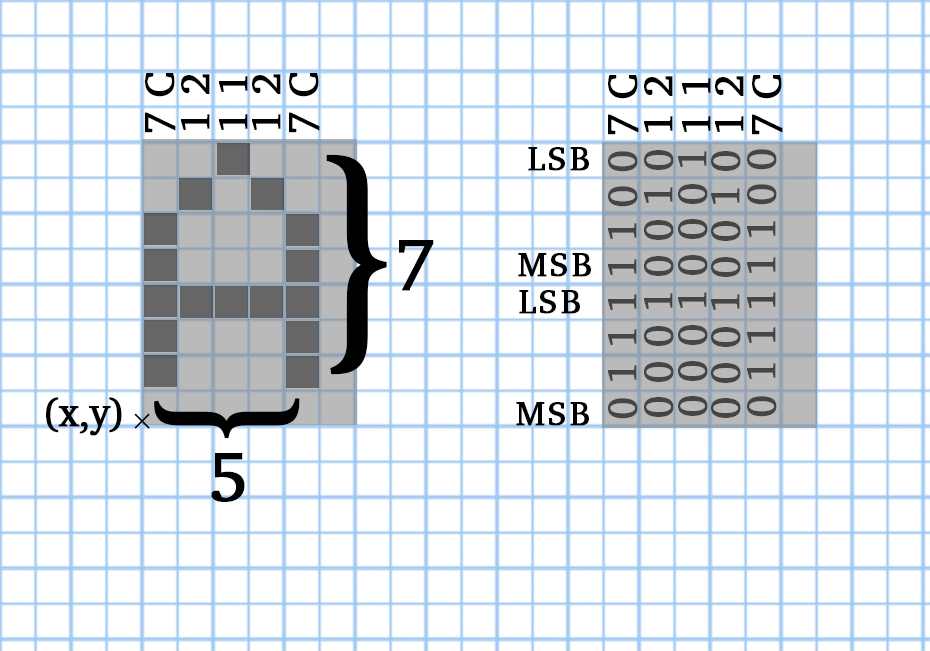
\includegraphics[width=.5\textwidth]{./05_c/figures/ASCII57.png}
		\caption{ASCII 5*7 Schriftart}
		\label{fig:ascii57}
	\end{centering}
\end{figure}
Zum Anzeigen von Buchstaben auf dem Bildschirm wird eine ASCII 5 * 7 Bibliothek verwendet. Diese besteht aus einem Array mit 255 Buchstaben, die jeweils aus f{\"u}nf 8-Bit gro{\ss}en Hexadezimalzahlen bestehen. Die 5 * 7 Bibliothek eignet sich f{\"u}r den 480 * 320 gro{\ss}en Bildschirm, da die Darstellung dier Schriftart mit einer Fl{\"a}che von 35 Pixeln f{\"u}r einen Buchstaben trotzdem sehr gut lesbar ist. Wenn man von einem 1 Pixel Abstand zwischen den Buchstaben ausgeht, passen auf das Display bis zu 3 200 Zeichen. Somit es ist m{\"o}glich l{\"a}ngere Textpassagen auf dem Bildschirm ohne Probleme abzubilden. Die Methode \texttt{drawChar} kann mit Hilfe der ASCII Schriftart Buchstaben an jeder Stelle des Bildschirms in verschiedenen abbilden. Zus{\"a}tzliche Parameter au{\ss}er der Position sind Schriftfarbe, -gr{\"o}{\ss}e und Hintergrundfarbe. Durch die setUp-Methode ist der Bildschirm so eingestellt, dass sich der Koordinatenurpsrung in der unteren linken Ecke des Bildschirms befindet.  

In display.h ist die Schriftart, welche in der Datei glcdfont.h im Array font abgelegt ist, bereits eingebunden. Um globale Grundeinstellungen für die Schriftart festzulegen, wurde bereits die Variablen cursorX, cursorY, textColor, textSize und textBackground deklariert. 

(1.) Implementiere die Set-Funktionen für die Variablen cursorX, cursorY, textColor, textSize und textBackground.

(2.) Die Funktion drawChar soll einen Buchstaben der ASCII-Schriftart auf dem Display an der Position x,y in der Farbe color mit der Hintergrundfarbe bg und der Größe size abbilden. Zunächst muss überprüft werden, ob die angegeben x,y Positionen im gültigen Wertebereich des Display liegen. Sofern die Werte die Grenzen des Bildschirms überschreiten, soll die Funktion drawChar beendet werden. Als nächster Schritt soll auf die richtige Stelle des Array font zugegriffen werden und die Bits der Hexadezimalwerte in Farbwerte intepretiert werden. Abbildung \ref{fig:ascii57} zeigt den Aufbau der Buchstaben im Array font am Beispiel von A. Jeder Buchstabe ist in font an der Position c*5 des Array gespeichert, wenn c für den ASCII-Wert des char steht. Für diesen Buchstaben werden 40 Bits durchiteriert und für jedes Bit, welches gleich 1 ist, wird an dieser Stelle ein Pixel oder Rechteck auf dem Display ausgegeben. Ist die Größe der Schriftart größer als 1, empfiehlt es sich statt drawPixel die Funktion fillRect zu verwenden. 

(3.) Um die Textausgabe auf dem Display für strings zu ermöglichen, müssen weitere Funktionen implementiert werden, die einen automatisierten Cursor verwenden, der die Position des letzten geschriebenen Buchstaben speichert. Die Funktion writeAuto(char c) soll die Aufgabe übernehmen einen Buchstaben c auf dem Display mit hilfe von drawChar zu schreiben und die Position der Cursor cursorX und cursorY zu verändern. Hierbei sind Display-Grenzen und Zeilenumbrüche zu beachten.

(4.) Implementiere die Funktion writeText(char *text), welche einen char Array als Parameter erhält und diesen mithilfe von writeAuto auf dem Display schreiben soll. Außerdem soll noch eine Abwandlung writeTextln(char *text) implementiert werden, welche am Ende des Strings noch einen Zeilenumsprung einfügen soll.

(5.) Zur Ausgabe von Zahlen soll die Funktion writeNumberOnDisplay(uint16\_t *value) implementiert werden, welche Integer in ein char-Array umwandelt und diesen mithilfe von writeText auf dem Display ausgibt. Die Funktion itoa aus der stdlib.h kann zur Lösung dieser Aufgabe hilfreich sein.
